\documentclass{beamer}
\usepackage{amsmath}
\usepackage{amssymb}
\usepackage{pgf}
\usepackage{tikz}
\usepackage{listings}
\usepackage{color}
\usetikzlibrary{matrix}
\usetheme{boxes}
\newcommand{\fig}{./figures} % common figure path
\newcommand{\msin}{\mbox{sin}} % math sin
\newcommand{\mcos}{\mbox{cos}} % math sin
\newcommand{\dbbslsh}{\textbackslash \textbackslash} % common figure path
\newcommand{\frnzplt}{FranzPlot }
\newenvironment{myblock}[3]{%
\definecolor{smtbx}{rgb}{0.64,0.76,0.68}
\setbeamercolor{block body}{#2}
\setbeamercolor{block title}{#3}
\begin{block}{#1}}{\end{block}}
\title[Curve e Sup. - Lab 5]{Curve e Superfici per il Design \\ Laboratorio 5 - Superfici parametriche}
\author[Prof.ssa Scotti]{Prof.ssa Anna Scotti}
%\institute[dimat]{Long Inst.}
\date{21 Maggio 2019}

\begin{document}
\lstset{language=POV}
\begin{frame}
\maketitle
\end{frame}
\section{Introduzione}
\begin{frame}
\frametitle{Materiali}
Nella con il materiale di oggi troverete:
\begin{itemize}
\item Questa presentazione (\texttt{lab5.pdf})
\end{itemize}
Troverete nella cartella Beep `FranzPlot-DCS':
\begin{itemize}
\item L'eseguibile \texttt{FranzPlot Launcher.exe}
\end{itemize}
Nella cartella `Materiale Laboratorio':
\begin{itemize}
%\item Il file \texttt{my\_include.inc}, che contiene delle macro necessarie per fare alcuni esercizi.
\item Il file trasformazioni\_ref.pdf.
\end{itemize}
\end{frame}
%
\section{Esercizi}
\begin{frame}
\frametitle{Esercizio 1: \textit{Surface} e \textit{Sample parameter}}
Data la superficie descritta dall'equazione
\begin{displaymath}
\begin{cases}
x(u,v) = \msin(u)\\
y(u,v) = \mcos(u) & u\in [0,2\pi], v \in[-1,1]\\
v(u,v) = v
\end{cases}
\end{displaymath}
\begin{itemize}
\item Rappresentare la superficie attraverso il nodo `Surface'.
\item Testare il  nodo `Sample parameter', che permette di nominare e
fissare un parametro di una superficie data, identificare le curve che si
ottengono fissando ad uno ad uno i  due parametri della superficie.  
\end{itemize}
\end{frame}
%
\begin{frame}
\frametitle{Esercizio 1 - i}
\begin{center}
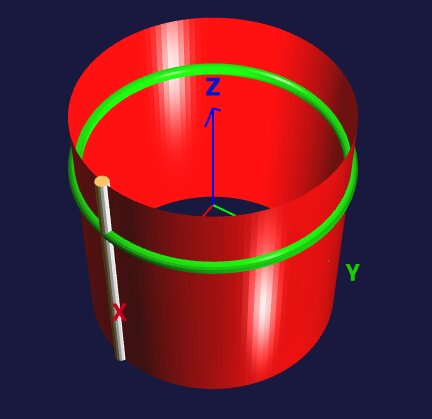
\includegraphics[width=0.8\textwidth]{\fig/l5_cyl_sampled.jpeg}
\end{center}
\end{frame}
%
\begin{frame}
\frametitle{Esercizio 2: Circonferenza $\rightarrow$ Cono}

Rappresentare un cono come traslazione e scalatura di una circonferenza

\begin{itemize}
\item Scrivere l'espressione della superficie trasformando la curva come indicato;
\item Rappresentare con \frnzplt la superficie e controllare che riproduca la
corretta trasformazione utilizzando le trasformazioni temporali della curva
(e$\backslash$ o il comando `Sample parameter').
%%%%
\end{itemize}
\end{frame}
%
\begin{frame}
\frametitle{Esercizio 2 -i }
\begin{columns}
\begin{column}{0.58\textwidth}
\begin{displaymath}
\mathcal{C}:
\begin{cases}
x = R~\mcos(u)\\
y = R~\msin(u), \;\;\;0\le u\le 2\pi\\
z = 0
\end{cases}
\end{displaymath}
\end{column}
\begin{column}{0.39\textwidth}
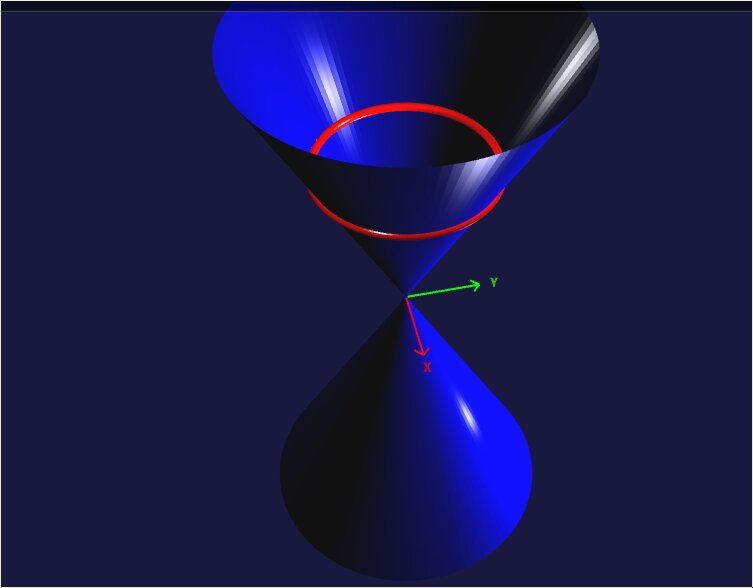
\includegraphics[width=0.8\textwidth]{\fig/l5_cone2.jpeg}

\end{column}
\end{columns}
%
\vspace{0.1\textheight}
\begin{displaymath}
\begin{bmatrix}
v/R & 0 & 0 & 0\\
0 & v/R & 0 & 0\\
0 & 0   & 1 & v\\
0 & 0   & 0 & 1
\end{bmatrix}
\cdot
\begin{bmatrix}
R~\mcos(u)\\
R~\msin(u)\\
0\\
1
\end{bmatrix}
= 
{\color{blue}
\begin{bmatrix}
v ~\mcos(u)\\
v ~\msin(u)\\
v\\
1
\end{bmatrix}
}
\end{displaymath}
\end{frame}
%
\begin{frame}
\frametitle{Esercizio 3: Circonferenza $\rightarrow$ Cilindro}
\begin{columns}
\begin{column}{0.58\textwidth}
\begin{displaymath}
\mathcal{C}:
\begin{cases}
x = R~\mcos(u) + x_0\\
y = R~\msin(u) + y_0, & 0\le u\le 2\pi\\
z = 0
\end{cases}
\end{displaymath}
\end{column}
\begin{column}{0.39\textwidth}
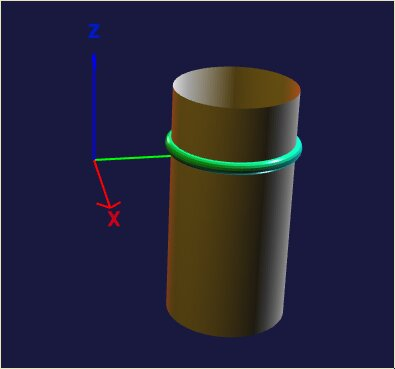
\includegraphics[width=0.8\textwidth]{\fig/l5_cyl.jpeg}

\end{column}
\end{columns}
%
\vspace{0.1\textheight}
\begin{displaymath}
\begin{bmatrix}
1 & 0 & 0 & 0\\
0 & 1 & 0 & 0\\
0 & 0 & 1 & v\\
0 & 0 & 0 & 1
\end{bmatrix}
\cdot
\begin{bmatrix}
R~\mcos(u)+x_0\\
R~\msin(u)+y_0\\
0\\
1
\end{bmatrix}
= 
{\color{blue}
\begin{bmatrix}
R ~\mcos(u)+x_0\\
R ~\msin(u)+y_0\\
v\\
1
\end{bmatrix}
}
\end{displaymath}
\end{frame}

\begin{frame}
\frametitle{Esercizio 3a: Cilindri deformati con tagli}
\begin{itemize}
\item Applicare la trasformazione che deriva da una traslazione in z di  $v$, seguita
da un taglio proporzionale a $v$ in direzione $x$ sulla superficie perpendicolare a
$z$. 
\end{itemize}
\begin{center}
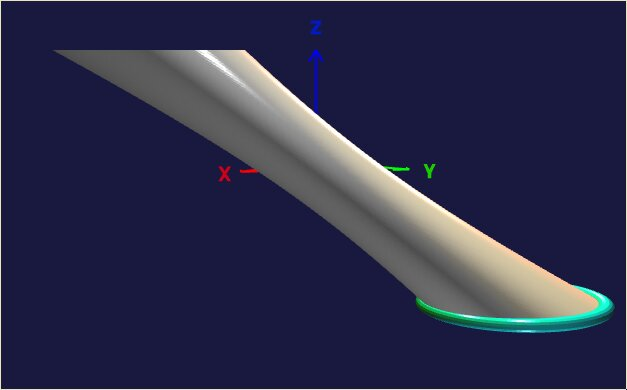
\includegraphics[width=0.6\textwidth]{\fig/l5_cyl_shear1.jpeg}
\end{center}
\end{frame}
\begin{frame}
\frametitle{Esercizio 3b:}
\begin{itemize}
\item Applicare alla stessa circonferenza una traslazione di $v$ in $z$,
seguita da un taglio proporzionale al parametro $v^2$ in direzione $x$ sul piano
con normale in direzione $z$.
\end{itemize}
\begin{center}
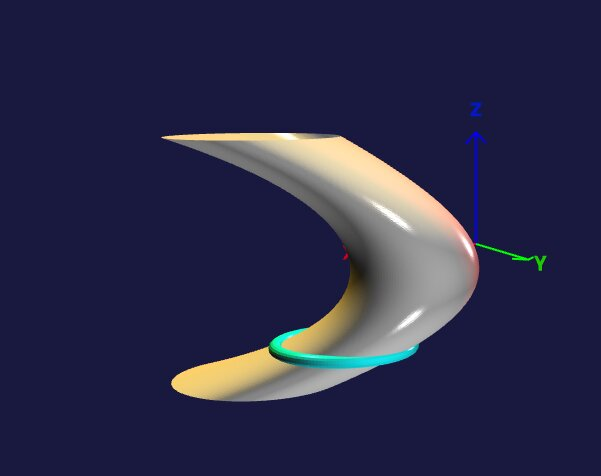
\includegraphics[width=0.6\textwidth]{\fig/l5_cyl_shear2.jpeg}
\end{center}
\end{frame}
\begin{frame}
\frametitle{Esercizio 4: Toro}
Nel caso sia ottenuto dalla rotazione di una circonferenza posta sul piano yz e ruotata attorno all'asse z:
\begin{center}
\begin{displaymath}
\begin{bmatrix}
\mcos(v) & -\msin(v) & 0 & 0  \\
\msin(v) &  \mcos(v) & 0 & 0  \\
0        &  0        & 1 & 0  \\
0        &  0        & 0 & 1
\end{bmatrix}
\cdot
\begin{bmatrix}
0 \\
h_1+R~\msin(u)\\
h_2+R~\mcos(u)\\
1
\end{bmatrix}
\end{displaymath}
\begin{displaymath}
={\color{blue} 
\begin{bmatrix}
-h_1~\msin(v)- R ~\msin(v)~\msin(u)\\
h_1~\mcos(v) + R~\mcos(v)~\msin(u)\\
h_2+R~\mcos(u)\\
1
\end{bmatrix}}
\end{displaymath}
\end{center}
\end{frame}
\begin{frame}
\frametitle{Esercizio 4 - i}
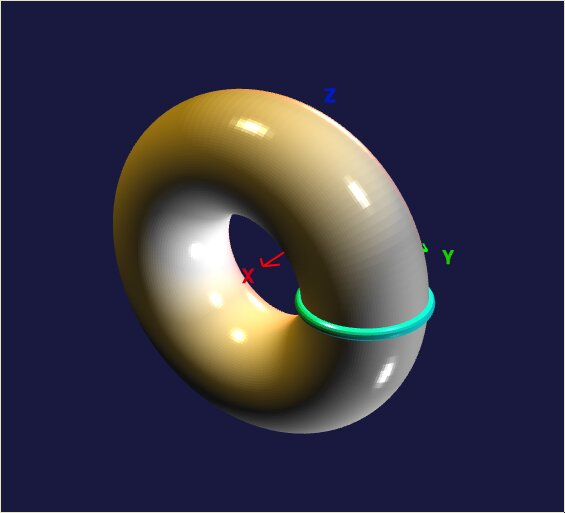
\includegraphics[width=0.8\textwidth]{\fig/l5_toro.jpeg}
\end{frame}

\begin{frame}
\frametitle{Esercizio 5: Ellissoide}
\begin{itemize}
\item Ricavare l'equazione di un ellissoide con semiassi \\
a = 2 (asse x), b = c = 1 (assi y e z);
\end{itemize}
\begin{columns}
\begin{column}{0.58\textwidth}
\begin{itemize}
\item Rappresentare la superficie con \frnzplt
\end{itemize}
\end{column}
\begin{column}{0.39\textwidth}
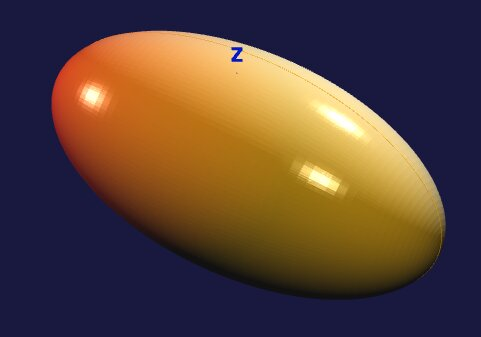
\includegraphics[width=\textwidth]{\fig/l5_ellipsoid.jpeg}

\end{column}
\end{columns}
%
\end{frame}
\begin{frame}
\frametitle{Esercizio 6}
Rappresentare con \frnzplt la seguente superficie:
\begin{columns}
\begin{column}{0.58\textwidth}
\begin{displaymath}
\Sigma:
\begin{cases}
x = u~\mcos(v)\\ 
y = u^2\\
z = u~\msin(v)
\end{cases}
\end{displaymath}
\begin{displaymath}
0\le u \le 2, \;\;\;\; 0\le v\le 2\pi
\end{displaymath}
\end{column}
\begin{column}{0.39\textwidth}
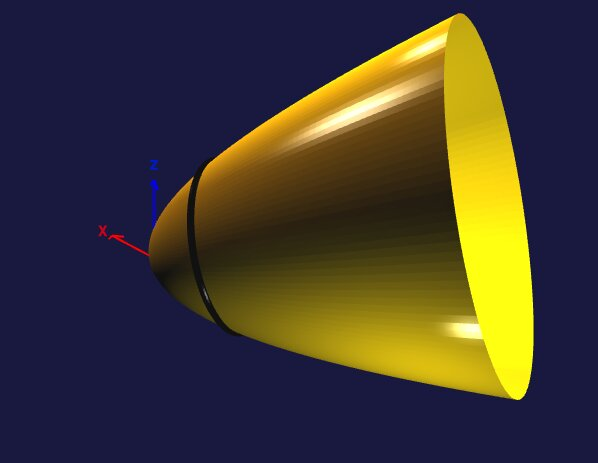
\includegraphics[width=\textwidth]{\fig/l5_parab.jpeg}
\end{column}
\end{columns}
\begin{myblock}{}{bg=smtbx,fg=black}{bg=smtbx, fg=red}
\begin{itemize}
\item Utilizzare il nodo `Sampling Parameter' come aiuto per identificare le curve che compongono la superficie.
\end{itemize}
\end{myblock}

%
\end{frame}
\begin{frame}
\frametitle{Per Casa:}
Le pagine seguenti contengono esercizi simili a quelli incontrati nella
precedente parte del laboratorio, con superfici gi\`a viste a lezione. 

\end{frame}
\begin{frame}
\frametitle{Esercizio A: Retta $\rightarrow$ Cono}
\begin{itemize}
\item Data  retta $r$, di equazione:
\begin{displaymath}
r:
\begin{cases}
x = 0 \\
y = 0.5~u\\
z = u
\end{cases}
\end{displaymath}
dove $u$ \`e il parametro.
\item Dedurre e rappresentare la curva ottenuta applicando una rotazione di $2\pi$ attorno all'asse $z$ di $r$.
\end{itemize}
\end{frame}
%%%
\begin{frame}
\frametitle{Esercizio A - i}
\begin{displaymath}
\begin{bmatrix}
\mcos(v) &  -\msin(v) & 0 & 0\\
\msin(v) &   \mcos(v) & 0 & 0\\
0 & 0 & 1 & 0\\
0 & 0 & 0 & 1
\end{bmatrix}
\begin{bmatrix}
0 \\ 0.5~u \\ u\\ 1
\end{bmatrix}
= 
\begin{bmatrix}
-0.5~u~\msin(v) \\ 0.5~u\mcos(v) \\ u \\ 1
\end{bmatrix}
\end{displaymath}
\end{frame}
%%%
\begin{frame}
\frametitle{Esercizio A - ii}
\begin{center}
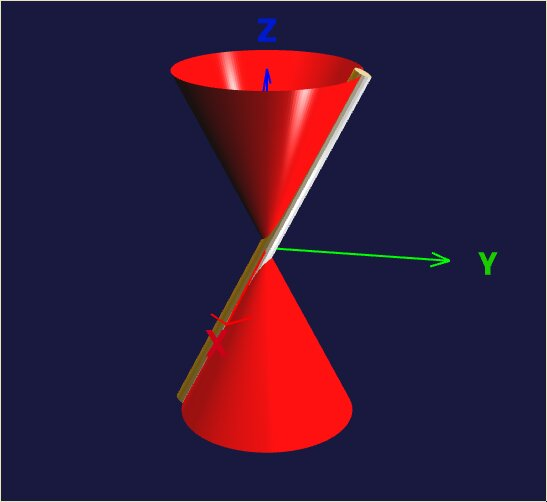
\includegraphics[width=0.8\textwidth]{\fig/l5_cone1.jpeg}
\end{center}
\end{frame}
%
\begin{frame}
\frametitle{Esercizio B: Retta $\rightarrow$ Cilindro}
\begin{columns}
\begin{column}{0.58\textwidth}
\begin{displaymath}
\mathcal{C}:
\begin{cases}
x = 0\\
y = 2\\
z = u
\end{cases}
\end{displaymath}
\end{column}
\begin{column}{0.39\textwidth}
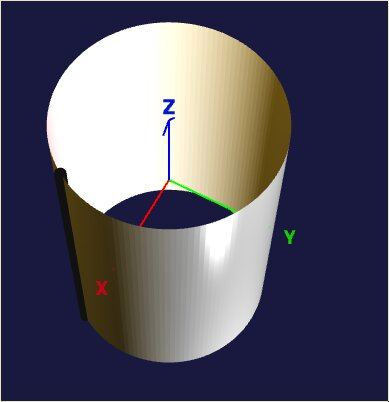
\includegraphics[width=0.8\textwidth]{\fig/l5_cyl_line.jpeg}

\end{column}
\end{columns}
%
\vspace{0.1\textheight}
\begin{displaymath}
\begin{bmatrix}
\mcos(v) & -\msin(v) & 0 & 0\\
\msin(v) &  \mcos(v) & 0 & 0\\
0        & 0         & 1 & 0\\
0        & 0         & 0 & 1
\end{bmatrix}
\cdot
\begin{bmatrix}
0\\
2\\
u\\
1
\end{bmatrix}
= 
{\color{blue}
\begin{bmatrix}
-2\msin(v)\\
2\mcos(v)\\
u\\
1
\end{bmatrix}
}
\end{displaymath}
\end{frame}
\begin{frame}
\frametitle{Esercizio C: Circonferenza $\rightarrow$ Sfera}
\begin{columns}
\begin{column}{0.58\textwidth}
\begin{displaymath}
\mathcal{C}:
\begin{cases}
x = R~\mcos(u)\\
y = R~\msin(u), \;\;\;0\le u\le 2\pi\\
z = 0
\end{cases}
\end{displaymath}
\end{column}
\begin{column}{0.39\textwidth}
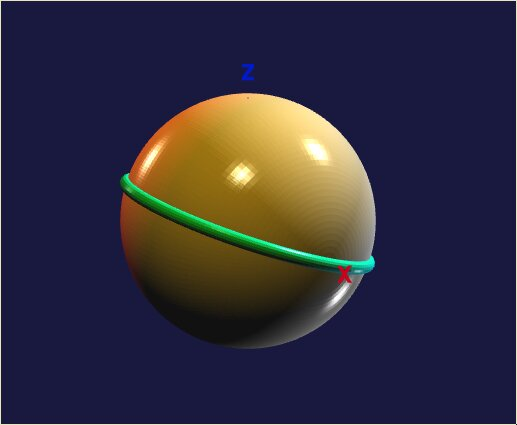
\includegraphics[width=0.8\textwidth]{\fig/l5_sphere.jpeg}

\end{column}
\end{columns}
%
\vspace{0.1\textheight}
\begin{displaymath}
\begin{bmatrix}
1 & 0 & 0 & 0\\
0 & \mcos(v) & -\msin(v) & 0\\
0 & \msin(v)   & \mcos(v) & 0\\
0 & 0   & 0 & 1
\end{bmatrix}
\cdot
\begin{bmatrix}
R~\mcos(u)\\
R~\msin(u)\\
0\\
1
\end{bmatrix}
= 
{\color{blue}
\begin{bmatrix}
R ~\mcos(u)\\
R ~\msin(u)~\mcos(v)\\
R ~\msin(u)~\msin(v)\\
1
\end{bmatrix}
}
\end{displaymath}
\end{frame}
\end{document}
